\documentclass[11pt,preprint,flushrt]{aastex}
\usepackage{amsmath}
\usepackage{amssymb}
\usepackage{latexsym}
\usepackage{cancel}
\usepackage{verbatim}
\usepackage{indentfirst}
\usepackage{multirow}
\usepackage{color}
\usepackage{graphicx}
\usepackage{multicol}
\usepackage{natbib}
\usepackage{hyperref}
\usepackage{graphicx}


%\usepackage[utf8]{inputenc}
 
%\setlength{\arrayrulewidth}{1mm}
%\setlength{\tabcolsep}{18pt}
%\renewcommand{\arraystretch}{1.5}


\begin{document}


\newcommand {\gs} {{\tt{GalSim}}}  
\newcommand {\wf} {WFIRST}  
\newcommand {\wfa} {WFIRST-AFTA}  
\newcommand {\optical} {{\tt{OpticalPSF}}} 
\newcommand {\gauss} {{\tt{Gaussian}}} 

%\def\dv{\mbox{$\Delta V$}}

\title{Voltage non-linearity effects on \wfa\ PSF profiles for weak lensing measurements using {\tt{GalSim}} simulations}
\author{A. A. Plazas$^{\dagger a}$, C. Shapiro$^a$, J. Rhodes$^a$, \& R. Smith$^b$}
\email{$^\dagger$andres.a.plazas.malagon@jpl.nasa.gov}
\affil{$^a$Jet Propulsion Laboratory, California Institute of Technology, 4800 Oak Grove Dr., Pasadena, CA 91109, USA}
\affil{$^b$Caltech Optical Observatories, 1200 E. California Blvd, MC11-17, CA 91125, USA}
\begin{abstract}
Weak gravitational lensing (WL) is one of the most powerful techniques to learn about the dark sector of the universe. To extract the WL signal from astronomical observations, observed galaxy shapes must be measured and corrected for the Point Spread Function (PSF) of the imaging system with extreme accuracy (of the order of 1 part per 1000). Future missions such as NASA's Wide Field Infrared Survey Telescope-Astrophysics Focused Telescope Asset (\wfa) will use a new family of hybrid near-infrared CMOS detectors that can potentially bias WL measurements. In particular, these detectors are intrinsically subject to non-linearities in the conversion of photo-generated charge to measured voltage that tend to attenuate bright objects such as reference stars that are used for PSF determination. In this paper, we study the impact on \wf\ PSF properties (size and ellipticity) induced by this type of signal-dependent voltage non-linearity (VNL). We use the publicly-available \gs\ and the \wf\ Exposure Time Calculator codes to generate customized simulations of the PSF optical profiles expected for \wf\ and study the consequences of a one-parameter non-linearity function quadratic in the signal $Q$ (in electrons) per pixel, $f(Q)=Q-\beta Q^2$. We use these simulations to measure the fractional error in the PSF size ($\Delta R/R$) and the absolute error in the PSF ellipticity ($\Delta e$) as a function of parameters such as the expected magnitude of typical stars in \wf\ and  $\beta$. For a measured nominal $\beta_0=3.566\times10^{-7}/e^{-}$, VNL attenuates the signal by about $3.5\%$ per each $10^5$ e$^-$ input. We find that the effect of VNL is chromatic in the four bands of the High Latitude Survey (HLS) of \wf\, and that its amplitude is the largest for the J129 band. As $\beta$ is allowed to increase, the values of $\Delta R/R$ and $\Delta e$ increase linearly in all bands at a fixed magnitude. We find that if not corrected, VNL at its nominal value can induce an error of $\Delta R/R=5\times 10^{-3}$ and $\Delta e_2=10^3$ in the \wf\ PSF size and ellipticity in the J129 bandpass for the expected brightest stars in the High Latitude Survey of \wf. In addition, or simulations show that to limit the bias of $\Delta R/R$ and $\Delta e$ in the J129 band to better than 1 part in 1000, $\beta$ must be calibrated to $\sim3\%$ and $\sim 6\%$, respectively.  
\end{abstract}

\section{Introduction}
Weak gravitational lensing (WL) has been identified as a powerful probe of the nature and evolution of the components of the Universe. In particular, \emph{cosmic shear}-the subtle  distortions of background galaxy shapes by the large scale structure of the Universe-constrains the properties of dark matter and dark energy through the measurement of the expansion history and growth of structure of the Universe\citep{refregier03, hoekstra08, kilbinger15}. In addition, WL measurements allow to test the validity of General Relativity that relates the gravitational potential to the matter-energy distribution. Several visible and near-infra red (NIR) surveys of $>1000$~deg$^2$ of the sky are currently underway and use the WL signal from hundreds of millions of galaxies as one of their central scientific techniques (\emph{e.g.}, the Dark Energy Survey (DES) \citep{diehl12,jarvis15}, the the Kilo-Degree Survey (KiDS) \citep{kuijken15}, and the Hypersuprime-Camera Survey (HSC)\citep{miyazaki12}. In addition, future ground- and spaced-based surveys and missions are planned to image more than O($10^9$) galaxies in the next decade (\emph{e.g.}, the Large Synoptic Survey Telescope (LSST) \citep{ivezic08}, the Euclid spacecraft \citep{laureijs11} and  NASA's planned Wide Field Infrared Survey Telescope (WFIRST) in its Astrophysics Focused Telescope Asset (AFTA) implementation \citep{green12,spergel13,spergel15}).

The process of extracting the WL signal from images of the sky, in the presence of intrinsic galaxy ellipticity variations are $\sim$ 0.4 r.m.s, is highly non-trivial. It must be done through an statistical analysis of large galaxy samples, with a careful control of systematic uncertainties. The dominant signal produced by WL can be described by a local linear transformation of the source image that produces a shear (a complex, spin-2 field of components $\gamma_1$ and $\gamma_2$) and a scalar magnification, both of which have an r.m.s. amplitude of only $\sim 2 \%$ in the case of cosmic shear. Most of the background galaxies usable by WL are at hight redshift (with low signal-to-noise (S/N) ratio) and with a size comparable or smaller than the Point Spread Function (PSF) of the imaging system. The PSF itself is usually larger than the lensing signal by an order of magnitude, inducing a modulation in the signal (multiplicative errors) and asymmetries that produce coherent spurious patterns (additive errors) that mimmic the WL signal. Bright stars are commonly used to estimate the PSF function, and then this information must be interpolated to the observed galaxy positions to deconvolve the PSF contribution and measure the galaxy shape (in the form of a complex ellipticity $e=e_1 + i e_2$) to estimate the shear field\footnote{Most of the shape measurement algorithms to date rely on the accurate measurements of galaxy shapes to produce an estimator of the WL shear field $(\gamma_1, \gamma_2)$. However, recent algorithms propose skipping this step and creating a direct shear estimator through Bayesian analysis in Fourier space \citep{bernstein14,bernstein15})}. This interpolation step is subject to introduce systematic errors if the information inferred from the stars does not fully constrain the PSF at the galaxy position with the required accuracy.  In order not to bias the determination of cosmological parameters and dark energy, the ellipticity and size of the PSF must be known to an accuracy of O(10$^{-3}$) \citep{huterer06,amara08,paulin08,paulin09,massey13,cropper13} or better ($4.7 \times 10^{-4}$ for the knowledgement of the \wfa\ PSF ellipticity  \citep{spergel13}). 

%Space-based measurements offer potentially enormous advantages for weak lensing because of high angular resolution and stability of the observing platform, allowing accurate characterization of the instrumental point spread function (PSF).

Systematic errors that originate from the photon detectors can also introduce biases in astronomical observables such as photometry and astrometry that propagate into shear measurement biases. These type of errors have been extensively studied in the case of thick, fully-depleted, high-resistivity CCDs, which are the detectors of choice for many current and planned surveys such as DES, HSC, and LSST \citep{stubbs14,plazas14,gruen15}. It is of great importance to qualitatively quantify the impact of these sensor effects on the inference of cosmological parameter, in particular through WL \citep{jarvis14,mandelbaum14b,meyers14}. Future missions such as the James Webb Space Telescope and \wfa\ will utilize a new family of near-infrared detectors that are subject as well to effects such as non-linearity, reciprocity failure \citep{biesiadzinski11}, interpixel capacitance (IPC) \citep{mccullough08,kannawadi15}, and persistence\citep{smith08}, and that can potentially imprint biases on weak lensing shape measurements if not taken into account. 

In this paper we study the effect on PSF size and ellipticity of the non-linearity in the conversion of photo-generated charge to measured voltages in the NIR detectors that will be used by NASA's \wfa\ mission. This voltage non-linearity (VNL) will tend to attenuate the flux in bright stars, broadening the PSF and complicating the deconvolution of the PSF from the observed galaxy image, which itself is fainter and less subject to the effects of VNL. We use the {\tt{python}}/{\tt{C++}} code \gs\footnote{\url{https://github.com/GalSim-developers}} \citep{rowe15} to create PSF profiles with the optical properties of \wfa\ to analyze the impact of VNL on PSF size and ellipticity. 

In Section \S2 we summarize the main characteristics of the NIR detectors that will be utilized in \wfa\, and discuss about VNL. In Section \S3 we describe the simulations we create to study VNL for \wfa\ PSF profiles. Section \S4 presents our main results on fractional errors in size and absolute errors in ellipticity caused by VNL, as function of relevant parameters such as mean non-linearity amplitude and PSF magnitude. We conclude in Section \S5 with a discussion of our results and how they can be use din the derivation of NIR detector specifications to satisfy WL accuracy requirements. 

\section{Voltage non-linearity in the NIR detectors of \wfa}
\label{section:vnl}
%\textcolor{red}{In this section we explain voltage non-linearity, and how it can affect WL science through PSF broadening. Cite the appropriate references from the literature (i.e., previous studies of VNL for these type of detectors). Roger's document on measurements and emails have many good explanations, and should be cited/paraphrased.}

%% There is an obvious potential for non-linearity between photon ?ux and output voltage in the photovoltaic detectors which is absent in CCDs, simply because the detector capacitance is not �xed, but does in fact depend on the width of the pn depletion region, which in turn depends on the value of the reverse bias voltage. (Variations in the size of the depletion region do occur in a CCD, but this is a small e??ect.) The bias voltage changes continuously as the cell integrates, irrespective of whether it is storing photogenerated charges or dark current charges.

%In general, how- ever, IR arrays are continuously exposed to light, and therefore the exposure time is controlled by the sequence of reset and read pulses.

% Sample Up The Ramp: 
%In this approach, the signal is sampled many times at regular intervals throughout the duration of the exposure, rather than multiple times at the beginning and at the end. Therefore, the signal can be seen to ``ramp'' up (Chapman et al., 1990; Garnett and Forrest, 1993)

%Each pixel of an HxRG array is a 3-T (three transistor) design with a source fol- lower MOSFET providing charge-to-voltage conversion.  The gate of the source fol- lower is connected to the detector pixel with an indium bump

%IPCInter-pixel capacitance (IPC): For CMOS arrays made with source follower (SF) pixels, the gate of the SF of one pixel is capacitively coupled to some degree to the SF in each of the 4 neighboring pixels. Since the voltage on a SF gate changes as photocharge is accumulated, this voltage change will modify the voltage on neighboring pixels, causing an electrical crosstalk between pixels. This crosstalk occurs after charge collection and during the charge-to-voltage conversion pro- cess. This ?inter-pixel capacitance? (IPC) can be conducted via three paths: (1) through the ROIC, (2) through the indium bumps, or (3) through the detector ma- terial. Since a silicon PIN detector is fully depleted, capacitive coupling through the detector material is dominant. For a H2RG, the IPC for a silicon HyViSI H2RG array is 8-10% to nearest neighbor.

%Non-linearity: A source follower is inherently non-linear, since the gate of the amplifier de-biases during charge integration. This leads to a roll-off of response as the detector approaches full well. Pixel full well is typically defined as the charge level at which the response is 5% deviation from linear, which is typically about 100,000 electrons for the HxRG designs (the exact number depends on the operating conditions)

The \wfa\ mission will use a 2.4-m telescope equipped with a Wide Field Instrument (WFI) with 6 bandpass filters (Z087, Y106, J129, W149, H158, and F184 \citep{spergel15})\footnote{In addition to a integral field unit and a coronagraph for supernovae and exoplanet studies, respectively} for constraining dark energy. The WFI will perform a high-latitude survey (HLS) over an area of 2200 deg$^2$ in four NIR ($\sim0.92 - 2.00 \mu$m) bands (Y106, J129, H158, and F184) down to a 5$\sigma$ point-source AB magnitude of 26.7 in J. The weak lensing program in the HSL will measure shapes of about 380 million galaxies in the J129, H158, and F184 \citep{green12,spergel15}

The WFI possesses a wide-field channel that has a Focal Plane Assembly (FCA) of 18 4k x 4k HgCdTe (mercury, cadmium, and telluride, or ``MerCadTel") Sensor Chip Assemblies (SCAs), arranged in a 6x3 layout and with a pixel size and plate scale of 10 $\mu$m and 0.11 arcseconds per pixel, respectively. The HgCdTe NIR detectors are manufactured by Teledyne Imaging Sensors, and are part of a family of detectors known as H4RG\footnote{``HAWAII 4k$\times$4k pixels with Reference pixels and Guide mode", where ``HAWAII" stands for HgCdTe Astronomical Wide Area Infrared Imager}. 

The detector arrays are fabricated with a hybrid complementary metal-oxid-semiconductor (CMOS) architecture, which combines the qualities of HgCdTe to detect IR light (\emph{e.g.}, altering the relative molar contributions of mercury and cadmium allows to tune the band gap up to an order of magnitude) and the advanced readout performance of integrated circuits. Light is absorbed, converted to charge through the photoelectric effect, and collected by electric fields generated by a reverse-biased p-n junction in the detector layer.  The charge per pixel is then converted to a voltage and amplified through a source follower. This operation is performed in the silicon readout integrated circuit (ROIC) layer, which is connected to the HgCdTe detection layer by indium interconnects (one bump per pixel). Finally, the ROIC transfers the signal (and for this it is also known as ``multiplexer") to the off-chip electronics at the edge of the FPA, where it is digitized through analog-to-digital converters \citep{beletic08}.

%The presence of the signal amplifier in each pixel causes a signal coupling among neighboring pixels (\emph{i.e.}, the charge in a pixel induces a voltage change in a neighbor) that is known as Inter-Pixel Capacitance (IPC). IPC is a type of crosstalk analogous to the amplifier crosstalk seen in multichannel CCDs (REFERENCE to O'Connor et al), and can have undesirable effects on PSF correction for WL science (REF ARUN et al). In addition to IPC, NIR detectors present other type of sensor effects that must be calibrated and/or corrected for accurate WL measurements. In particular,  

An ideal detector would produce a measurable signal that is proportional to the detected photons. However, there are several places in the signal chain where this expected linearity is not realized, and the conversion of charge to measured voltage (or analog-to-digital units, ADU) becomes non-linear. First of all, the charge accumulation rate might be a function of the photon-accumulation rate. This type of effect is known as reciprocity failure (RF), and it is a flux-dependent non-linearity (\citet{smith08}, \citet{biesiadzinski11}). In addition to RF, the p-n junction acts as a parallel-plate capacitor, and as charge accumulates the depletion region narrows, causing a deviation from linearity of the charge-to-voltage conversion relation. Non-linearity can also be introduced through the electronic gain of the ROIC. 

The last two types of non-linearity depend on fluence (total flux per pixel, or integrated signal, as opposed to RF, which is flux dependent), and can be analyzed together in a singe transfer function known as \emph{voltage non-linearity} (VNL). We study the impacts of VNL (more relevant at high signals) on PSF measurements in this paper, while we leave investigations on the consequences of RF (relevant at lower signals) on WL measurements for future work. 

Laboratory measurements with a H2RG detector (similar to the H4RG that will be used in the WFI) show that the voltage relation for a measured signal S is well fit by a quadratic function in the \emph{average} signal $\langle Q \rangle$ of the form:
\begin{align}
S(\langle Q \rangle)=\langle Q \rangle-\beta \langle Q \rangle^2 \ \ (e^{-})
\label{vnl}
\end{align}
We \emph{assume} that each individual pixel satisfies a VNL function of the same form as Eq. \ref{vnl}, and that the spatial variation on VNL is such as the non-linearity coefficient $\beta$ in each pixel can be drawn from a Normal distribution of the form $\mathcal{N} \sim (\beta_0, 0.12\beta_0)$, where the nominal value $\beta_0 \equiv 3.566\times10^{-7}/e^{-}$ and the dispersion parameter of the distribution (RMS$=0.12\beta_0$). This mean nominal value implies an attenuation of the signal of about $3.5\%$ per each $10^5$ e$^-$ of input signal (Eq. \ref{vnl}). We assume that galaxies will have about two orders of magnitude less total electrons than bright stars, and therefore for this quadratic model, star shapes are distorted by VNL and galaxies are (approximately) not, which would result in incorrect PSF correction if not accounted for.  We have verified that the results using the mean VNL coefficient for all pixels do not differ significatively from those using the distribution above for each pixel. 

We apply this mapping to simulated \wfa\ PSF profiles and quantify the impact on PSF properties such as size and shape. 

\section{Methods}
\label{methods}
\subsection {Simulations}
We use the publicly available {\tt{GalSim}} code (v.13) to simulate the impact of VNL on the \wfa\ PSF shape and size. {\tt{GalSim}} is a {\tt{python/C++}} open-source code that allows the user to create simulations of astronomical objects, and it is especially useful in weak lensing investigations. 

\citet{kannawadi15} have developed within \gs\ (v1.3) a \wfa\ module called ``{\tt{galsim.wfirst}}", which allows the simulation of a PSF profile according to the optical design characteristics of the \wfa\ WFI \citep{pasquale14})\footnote{\citet{pasquale14} discuss the so-called ``Cycle 4" optical design, whereas the \gs\ \wfa\ module -used in this work- uses files corresponding to ``Cycle 5"}) through the calling of {\tt{galsim.wfirst.getPSF}} routine. This routine returns a {\tt{python}} dictionary of {\tt{galsim.ChromaticOp-}}\\{\tt{ticalPSF}} objects indexed by each one of the 18 H4RG SCAs of the FPA. It uses the optical configuration of the pupil plane to simulate PSF images in any \wfa\ WFI bandpass filter, with expected optical aberrations approximated as a linear combination of Zernike polynomials (up to Noll order equal to $11$, \citet{noll67}). For this work, we have created simulations in the four bands of the HLS (see Table 1).  A central circular obscuration ($30 \%$) and six support struts are included as well. The pupil plane configurations and Zernike models are publicly available.\footnote{\url{http://wfirst.gsfc.nasa.gov/science/sdt_public/wps/references/instrument/}} 

The current version of the module does not include PSF variations within the detector, and the PSF returned corresponds to that at the center of the SCA. In addition, the module assumes that the pupil plane configuration of all the six bands is the same and equivalent to that of the ``red" bands (\emph{i.e.}, W149, H158, and F184), and that the struts are not, in general, radial nor evenly spaced. However, these last two assumptions can be relaxed to expedite calculations, and the optional keyword {\tt{approximate\char`_struts}} can be set to {\tt{True}}. The module generates PSF models that do not include pointing jitter nor charge diffusion.  

For the simulations in this work, SCA number 18 was selected, which was found to have the largest intrinsic ellipticity (see below for a description of the shape measurement method utilized) across all bands among all the SCAs (Table 1). Aberrations such as defocus, astigmatism, coma, and line-of-sight motion patters couple to propagate into terms that produce azimuthally asymmetrical profiles. We also evaluate the PSF at the mean wavelength weighted by each bandpass or effective wavelength, and set the {\tt{approximate\char`_struts}} keyword to {\tt{False}} when creating the profile. We then form an effective PSF by convolving the profile with a 2D box car profile of length equal to the nominal plate scale of the \wfa\ WFI ({\tt{galsim.wfirst.pixel\char`_ scale$=0.11$}} arcseconds per pixel). 

%Table 1
\begin{table}[!htb]
\centering
\begin{tabular}{ |c| c | c| c| c| c| c | c|}
\hline
\multirow{2}{*}{Band} & Min. $\lambda$ & Max. $\lambda$ & $\lambda_{\text{eff}}$ & k($\lambda$) & e$_1$ & e$_2$ & $\sigma$ \\
& ($\mu$m) & ($\mu$m) & ($\mu$m) & (e$^{-}$) &  (SCA$=$18) & (SCA$=$18) & (pix) (SCA$=$18)  \\
\hline 
Y106 & 0.900 & 1.010 & 0.873 & 3.4470$\times10^4$ & 0.00841  & 0.2010 & 4.4455 \\
J129  & 1.095 & 1.500 & 1.292 & 9.5477$\times10^4$  & 0.00793 & 0.1313 & 4.5140 \\
H158 & 1.340 & 1.830 & 1.577 & 9.5178$\times10^4$  & 0.00790 & 0.0807 & 4.8340 \\
F184 & 1.630 & 2.060 & 1.837 & 7.1792$\times10^4$  & 0.00592 & 0.0557 & 5.2781 \\
\hline
\end{tabular}
\caption{The first column lists the four bands that will be used in the HLS. For weak lensing analysis, multi-band shape measurement will be done in J129, H158, and F184. Columns 2, 3, and 4 show their minimum, maximum, and effective wavelengths, respectively (from \citet{kannawadi15}). Column 5 shows the baseline flux (in electrons) $k(\lambda)$ of Eq. \ref{flux} at AB magnitude 20 as calculated by the ETC-WL, using the parameters defined in the Appendix. The last three columns show the ellipticity components and size of the \wfa\ PSF profile in SCA number 18 as calculated by the adaptive moments routine in \gs. SCA 18 was found to possess the largest values of absolute PSF ellipticity.} \label{table:1}
\end{table}

The resulting PSF profile created in this way will be undersampled (in accordance with the \wfa\ WFI design). In order to maximize the field of view, detectors in instruments of space missions are usually built with a physical size that results in undersampled images, which fail to satisfy the Nyquist-Shannon criterium for the maximum band limit set by the optical response of the system, and therefore produce aliased images.\footnote{The Nyquist-Shannon criterium states that the sampling interval $p$ must satisfy $p < 1/(2 u_{max})$, where $u_{max}$ is the highest frequency in the signal, in order to avoid aliasing.} In general, it is not possible to recover all the information of a continuous function from a discrete sample of points if the image is aliased, and measurements of astronomical object's properties such as magnitude and shape will be erroneous \citep{lauer99a,fruchter11,rhodes07}. 

To overcome this problem in real data, multiple dithered exposures are taken, and then put together by means of an image combination algorithm \citep{lauer99b,fruchter02,bertin06,rowe11} in order to produce an oversampled image that satisfies the Nyquist-Shannon criterium. 

To study VNL with simulations, however, it is not necessary to make use of such external software to produce an image at higher resolution. \gs\ objects can be drawn at a high resolution by using the method {\tt{galsim.GSObject.drawImage}}\footnote{The keyword {\tt{method}} should be set to {\tt{`no\char`_pixel'}} when calling {\tt{galsim.GSObject.drawImage}}, since by default it convolves its argument profile with a boxcar of length {\tt{pixel\char`_scale}}. This extra convolution must be turned off because the effective PSF profile we create already includes this pixel response.} and setting the parameter {\tt{scale}} to $p/N$, where $N\in \mathbb{Z}^{+}$ and $p$ is the native pixel scale. Thus, it suffices to apply the effect of VNL to the convolved PSF profile at its native scale, and then render it with a resolution $p/N$. 
In order to produce an oversampled image, the Nyquist-Shannon criterium implies that $N$ must be given by (see \emph{e.g.}, \citet{shapiro13})
\begin{align}
N=\frac{2p}{\lambda_{min} F}
\end{align}
where $p$ is the pixel size, $\lambda_{min}$ is the shortest wavelength in a given filter, and $F$ is the the f-number of the telescope. In the case of the \wfa\ telescope, $p=10\ \mu$m and $F=7.8$, resulting in $N\geq3$ for the J129 band. We have set $N$ equal to $6$ for our simulations. 

%However, we oversample the images at  the error due to discretizing, and to reduce the variance due to any sub-pixel offsets that PSFs may have. We have set $N$ equal to $6$ for our simulations.

Notice that this method to produce oversampled images can only be used in the case of sensor effects such as VNL, which only depend on each pixel individually. In the case of other effects that correlate the signal in one pixel with the signal of its neighbors (such as IPC), the effect should be applied to the native scale of the detector and then a properly sampled image should be generated through appropriate combination of several dithered images before performing any analysis (see for instance the ``interleaving" algorithm of \citet{kannawadi15}, also included in \gs). 

\begin{figure}[!h]
\centering
\resizebox{\hsize}{!}{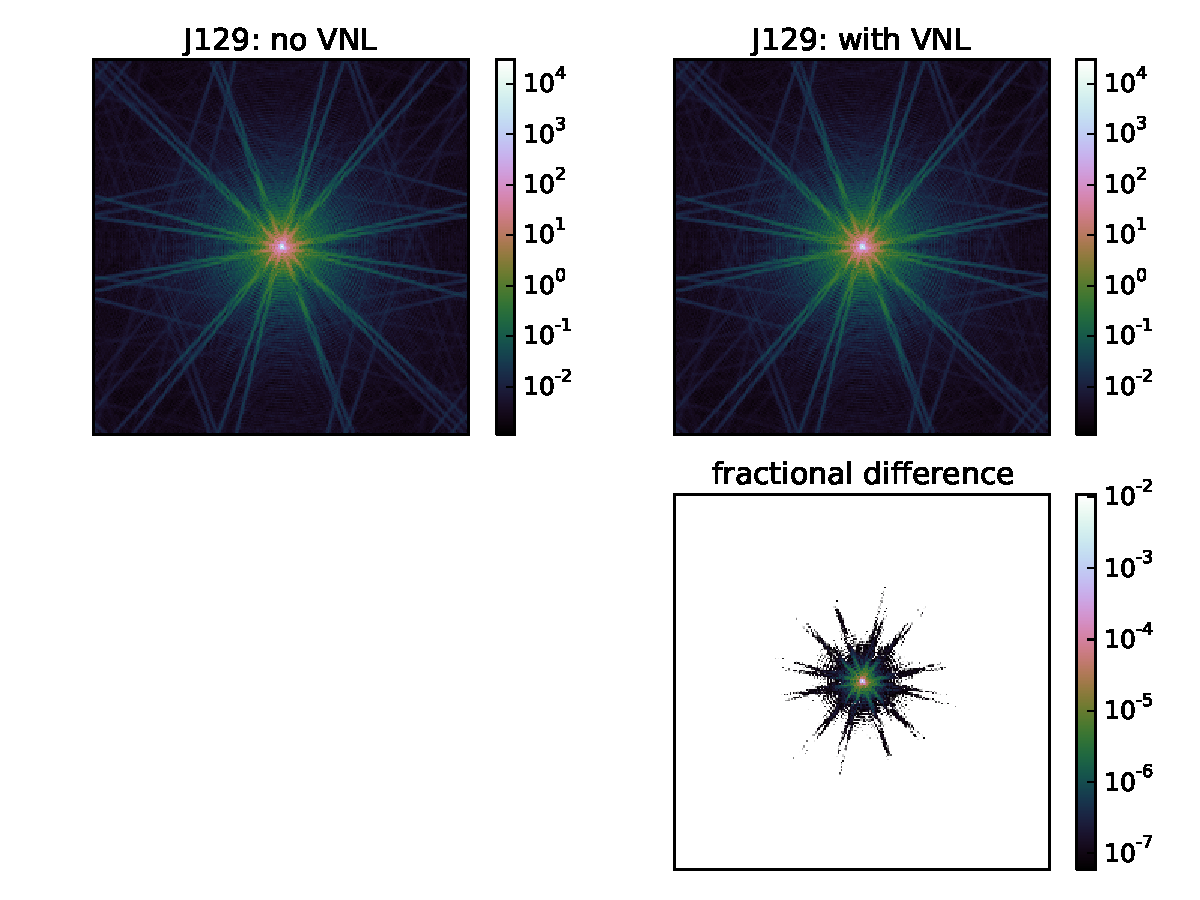
\includegraphics[page=1]{plots/wf_psf_image.pdf}}
\caption{Example of the \wfa\ PSF profiles in the J129 band created by the {\tt{galsim.wfirst.getPSF}} method. Each postage stamp has a size of 2048$\times$2048 pixels, and is drawn at a resolution of $p/N$, with $p=0.11$ arcseconds and $N=6$. Before drawing the profiles, they are first convolved with a pixel response of size $p$ and given a flux according to the  ETC-WL (with the parameters of the Appendix) at an AB magnitude of 20 ($9.5477\times10^4\ e^{-1}$, Table 1). However, to preserve the right response to VNL, the higher-resolution image has $N^2$ more total flux. The VNL effect is applied at the native pixel scale $p$. Diffraction spikes and structures can be seen due to the optical properties and aberrations of the PSF model used. The upper left panel shows the PSF without the VNL applied, while the upper right panel has VNL with a nominal $\beta_0=3.566\times 10^{-7}/e^{-}$. The fractional difference between the two cases-of the order of 1\% (in the core pixels which have more flux)-is better appreciated in the image of the lower panel.}
\label{psf_image}
\end{figure}

The PSF profiles are drawn into square postage stamps of size $2048$ pixels, large enough to ensure that  all the flux applied to the original profile object is conserved when drawing the image. in addition, this avoid biases in PSF determination arising from object selection and deblending. Each profile object was assigned a total flux of 
\begin{align}
f=k(\lambda)\times2.521^{(20-m)} \ e^{-}, 
\label{flux}
\end{align}
which is the number of source counts per exposure and where $m$ represents the AB magnitude of the object. $k(\lambda)$e$^{-}$ is a baseline flux at AB magnitude $m=20$ determined by using the \wfa\ Exposure Time Calculator (\citet{hirata12}) in weak lensing mode (ETC-WL). Among other parameters, the flux depends on each bandpass filter, and its values are listed in \ref{table:1} for the particular set of parameters of the listed in the Appendix. The brightest magnitude used was AB $m=20$, based on the number of source counts in the J129 band calculated by the ETC-WL ($\sim 9.5477\times10^{4}$ electrons, representing about $86\%$ of the typical full well depth of the H4RG detectors of $\sim 1.1\times10^{5}$ electrons).\footnote{Dave Content (GSFC), private communication.}  However, since VNL is a function of signal, the total flux in the higher resolution image must be multiplied by a factor of $N^2$ to preserve the appropriate response per pixel to this effect, correcting for the fact that the new image has an equal number of more pixels than the one created at the native scale. 

To better study the consequences of VNL, the postage stamps are noiseless and no other sensor effect is applied. VNL is then (after convolving with a pixel of the size of the native scale) by using Eq. \ref{vnl} through the use of the {\tt{galsim.image.applyNonlinearity}} method. 

 Fig. \ref{psf_image} shows an example of the PSF profiles and postage stamps created for our simulations (J129 band). The effect of VNL (at the nominal $\beta_0$) is small, and the difference image reveals that the attenuation in the flux is of the order of a few percent, mainly for the larger signals found at the core of the PSF.  \citet{kannawadi15} present more details on the {\tt{galsim.wfirst}} module, along with examples of the profiles that can be generated in all 6 \wfa\ filters. 
\subsection {PSF size and shape measurement}
The accurate determination of PSF properties such as size and ellipticity is crucial to avoid the propagation of systematic biases in cosmological parameters through the use of weak gravitational lensing \citep{paulin08,paulin09,massey13,cropper13}. In general, the problem of galaxy and PSF shape measurements for accurate weak lensing is non-trivial, and even when the PSF is perfectly known, shape measurement algorithms can introduce biases. Several shape measurements algorithms--ranging from model-fitting methods to particular combinations of weighted central moments--have been and are being investigated in order to produce accurate shear estimators that satisfy the requirements of current and future WL surveys \citep{mandelbaum14a}.

To measure the profile shapes and size, we use the adaptive moments method \citep{bernstein02,hirata03}, which is already implemented in \gs\ as {\tt{galsim.hsm.Find-}} \\{\tt{AdaptiveMom()}}. Adaptive moments are effectively weighted by an elliptical Gaussian. At first they are calculated by computing moments weighted by a circular Gaussian with some arbitrary size. Then the output moments are used to define a new elliptical Gaussian that will act as a new weight function. The process is iteratively repeated until the output moments are the same as those of the weight function. The ellipticity $e=e_1 + ie_2$ and size $r$ are then defined as
\begin{align}
e_1&=\frac{\mathbf{I}_{xx} - \mathbf{I}_{yy}}{\mathbf{I}_{xx}+\mathbf{I}_{yy}} \\
e_2&=\frac{2\mathbf{I}_{xy}}{\mathbf{I}_{xx}+\mathbf{I}_{yy}} \\
r&=\det[\mathbf{I}]^{1/4}
 \end{align}
where the centroid $\mathbf{\bar{x}}$ and moment matrix $\mathbf{I}$ of an image are defined as
\begin{align}
\mathbf{\bar{x}}&=\frac{\int d^2\mathbf{x}\ w(\mathbf{x}) \mathbf{x} I(\mathbf{x})}{\int d^2 \mathbf{x}\ w(\mathbf{x})I(\mathbf{x})} \\
\mathbf{I}_{ij}&=\frac{\int d^2\mathbf{x}\ (\mathbf{x} - \mathbf{\bar{x}})_i  (\mathbf{x} - \mathbf{\bar{x}})_j w(\mathbf{x}) I(\mathbf{x})} {\int d^2\mathbf{x}\ w(\mathbf{x})I(\mathbf{x})}
\end{align}
for an elliptical Gaussian weight function $w(\mathbf{x})$. 

\subsection{Changes in size and ellipticity induced by VNL}
We quantify the effect of voltage non-linearity by measuring the fractional change in size and the absolute change in ellipticity of the PSF profiles, in the 4 filters of the HLS of \wfa\, and for several values of the VNL parameter $\beta$. We calculate the quantities $\Delta e_1$, $\Delta e_2$, and $\frac{\Delta R}{R}$, which are defined as the difference between the measured ellipticity or size after the effect (VNL) is applied and the reference values measured before (represented by the subscript ``$0$") the application of VNL:
\begin{align}
\Delta e_{i} &\equiv e_{i} - e_{i,0},\ \ \ i\in[1,2]  
\label{delta_e}
\end{align}
\begin{align}
\frac{\Delta R}{R} &\equiv \frac {{R} - R_{0}}  { R_{0}}
\label{delta_r}
\end{align}
In this way, we minimize the details and possible biased induced by the shape measurement algorithm, and concentrate only on the relative changes induced by the detector anomalies. 

The basic process is summarized by the following steps:  
\begin{itemize}
\item[1.] Create a \wfa\ PSF surface brightness profile with a given flux as prescribed by Eq. \ref{flux}. 
\item[2.] Convolve the PSF profile with a squared pixel response with the size of the native plate scale of the \wfa\ FPA ($p=0.11$ arcseconds per pixel) to produce an effective PSF. 
\item[3.] Draw the effective PSF profile in a noiseless postage stamp of size 2048 by 2048 pixels at a higher resolution of of $p/N$, with $N=6$, and multiply the resulting image by $N^2$. In this step, VNL is not yet applied, but it will be done so in a later step, so the flux still needs to be adjusted. 
\item[4.] Use the adaptive moments algorithm to measure the shape $e=(e_{1,0},e_{2,})$ and size $R_0$ of the profile to have as baseline reference.
\item[5.] Create another image of the effective PSF at a higher resolution and with the flux adjusted as in 3. To apply VNL, draw a $\beta$ from the distribution $\mathcal{N} \sim (\beta_0, 0.12\beta_0)$ for each pixel in the high-resolution image $I$, and apply the voltage non-linearity to the postage stamps according to the transformation $I \mapsto I - \beta I^2$ (\emph{c.f.} Eq. \ref{vnl}.)
\item[6.] Measure the shape and size of the object with the sensor effect applied, and calculate the quantities $\Delta e_1$, $\Delta e_2$, and $\frac{\Delta R}{R}$, as defined in Eqs. \ref{delta_e} and \ref{delta_r}. 
\item[7.] Repeat steps 5 and 6 for $M$ realizations of the $\beta$ distribution, and calculate the mean value of Eqs. \ref{delta_e} and \ref{delta_r} over all $M$ realizations. The error bars will be given by the standard error of the mean. In our simulations, we use $M=10$. 
\item [8.] Repeat  steps 1 to 7 for different AB magnitudes (fluxes) at fixed mean $\beta$ and for different VNL parameters at a fixed magnitude. 
\end{itemize}
\section{Results}
Fig. \ref{beta} shows the fractional change in PSF size and the absolute error in PSF ellipticity as a function of the nonlinearity parameter $\beta$, for different bandpass filters at fixed AB magnitude of 20, consistent with the magnitude of brightest stars that will be usable for the HLS. The effect has a chromatic dependence, with the amplitude being the largest in the J129 bandpass filter. 
\begin{figure}[!h]
\centering
\resizebox{\hsize}{!}{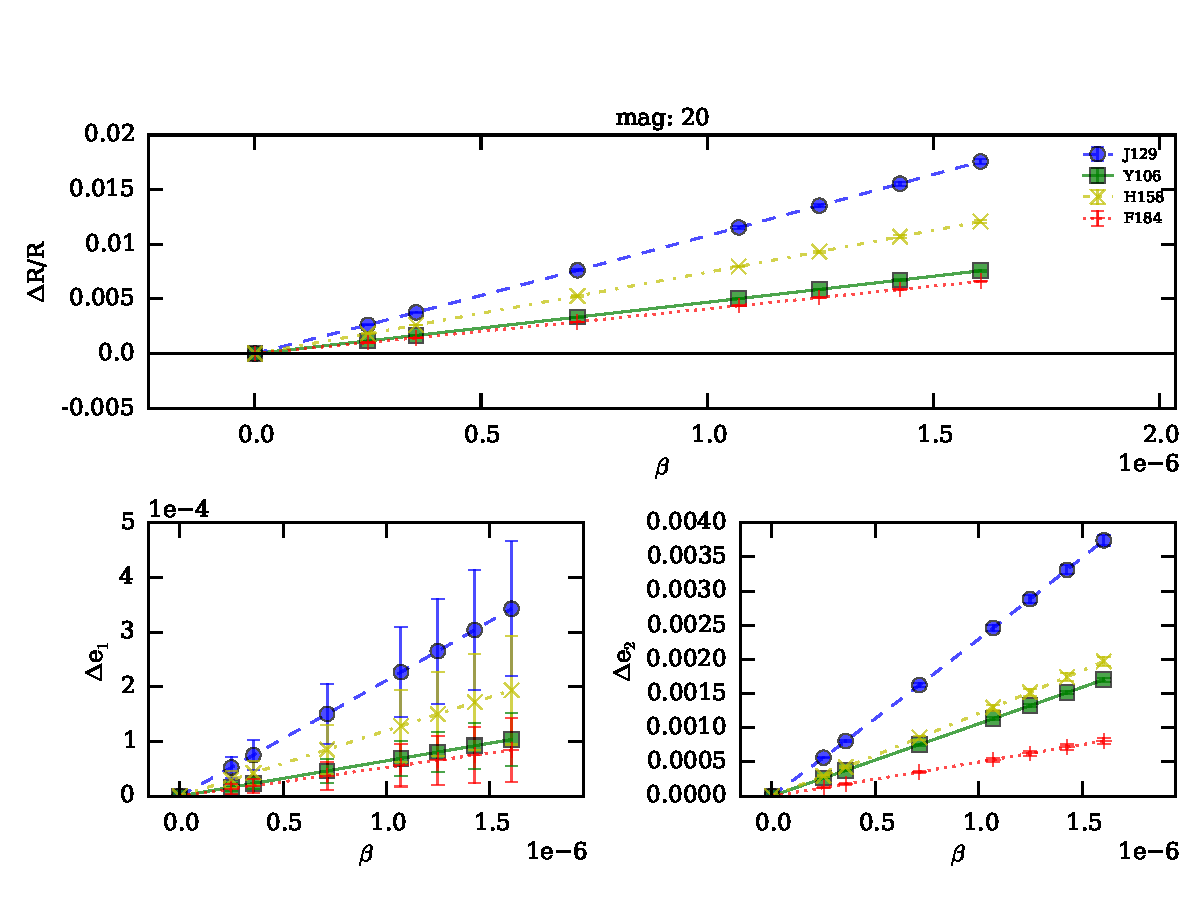
\includegraphics[page=1]{plots/delta_r_over_r_delta_e_mag20_wfirst_psf_10_realizations_12-13-2015.pdf}}
\caption{Fractional error in PSF size (upper panel) and absolute error in PSF ellipticity components (lower panels) as a function of nonlinearity parameter $\beta$ for the \wfa\ PSF, in four the four HSL filters (J129, Y106, H158, and F184), and an AB magnitude of 20 (similar plots were found for other values of magnitude). In each plot, the nominal value for the nonlinearity parameter as given by laboratory measurements, $\beta_0$, is located at the third point from the origin. Each point is the mean over $M=10$ realizations of the parameter $\beta$ per pixel, and the associated error bars (too small to be seen in the cases of $\Delta R/R$ and $\Delta e_2$) represent the standard error of the mean.}
\label{beta}
\end{figure}
In this band, the nominal value of $\beta_0=3.566\times10^{-7}/e^{-}$ induces errors in the size and ellipticity of about $5\times10^{-3}$ and $8\times10^{-4}$ respectively, comparable or even larger than the required values of $10^{-3}$ and $4.5\times10^{-4}$ on the knowledge of the size and ellipticity of the PSF in order not to bias cosmological parameter inferences from WL experiments (Section \S1). As the $\beta$ parameter is increased, the amplitude of the errors increases approximately in a linear manner within the domain of $\beta$ vales considered. 

It is possible to obtain a more general relationship between $\Delta R/R$ (or $\Delta e$), $\beta$, and object flux for each band by Taylor expanding to first order around any given value in $\beta$ and plotting the slope as a function of magnitude. This is shown in Fig. \ref{magnitude}, which shows $\Delta R/R/\beta$ and $\Delta e/\beta$ (the slopes in Fig. \ref{beta}) vs $m$ for each of the four filters of the HLS. From Fig. \ref{magnitude}, it is possible to estimate the precision to which $\beta$ would have to be calibrated in order to limit the relative size and ellipticity bias of a star with a given magnitude. In particular, letting $(\beta - \beta_0)/\beta_0 \equiv \Delta \beta / \beta_0$ represent the fractional error in the measurement of a given value of $\beta_0$ (which could differ from the $3.566\times 10^{-7}/e^{-}$ that we have been using so far), we have: 
\begin{align}
\frac{\Delta R/R}{\Delta \beta} = c \ \ \ \  \Rightarrow \ \ \ \ \frac{\Delta R/R}{\Delta \beta / \beta_0} = c \beta_0  \ \ \   \Rightarrow \ \ \
\frac{\Delta \beta}{\beta_0} = \frac{\Delta R/R}{c \beta_0}
\label{calib}
\end{align}
In Eq.\ref{calib}, $c$ represents the ordinate value in Fig. \ref{magnitude} for a given magnitude, and we have replaced $\Delta R/R/\beta$ by $\Delta R/R/ \Delta \beta$ since the linearity in the bias in $\Delta R/R$ and $\Delta e$ vs $\beta$ for all magnitudes makes the choice of the expansion point of the Taylor expansion unimportant (\emph{i.e.}, it does not matter if the expansion is around $\beta=0$ or $\beta=\beta_0$). An analogous equation to Eq.\ref{calib} can be written for the error in the ellipticity if $\Delta R/R$ is replaced by $\Delta e$. 

Under this conditions, Fig. \ref{magnitude} shows that to limit the bias of $\Delta R/R$ ($\Delta e$) in the J129 band to $10^{-4}$  ($4.7\times 10^{-5}$) \footnote{Ten percent of the estimated budget of $10^{-3}$ and $4.7 \times 10^{-4}$ in the knowledge of the PSF size and ellipticity, \emph{c.f.}, Section \S1}, $\beta$ must be calibrated to $\sim3\%$ ($\sim 6\%$) (using $c\sim10^4 e^{-}$ at $m=20$ from the upper panel of Fig. \ref{magnitude}, $c\sim2500$ at $m=20$ from the lower right panel of the same figure, and $\beta_0=3.566\times10^{-7}/e^{-}$) for the brightest stars usable by the HLS. 
\begin{figure}[!h]
\centering
\resizebox{\hsize}{!}{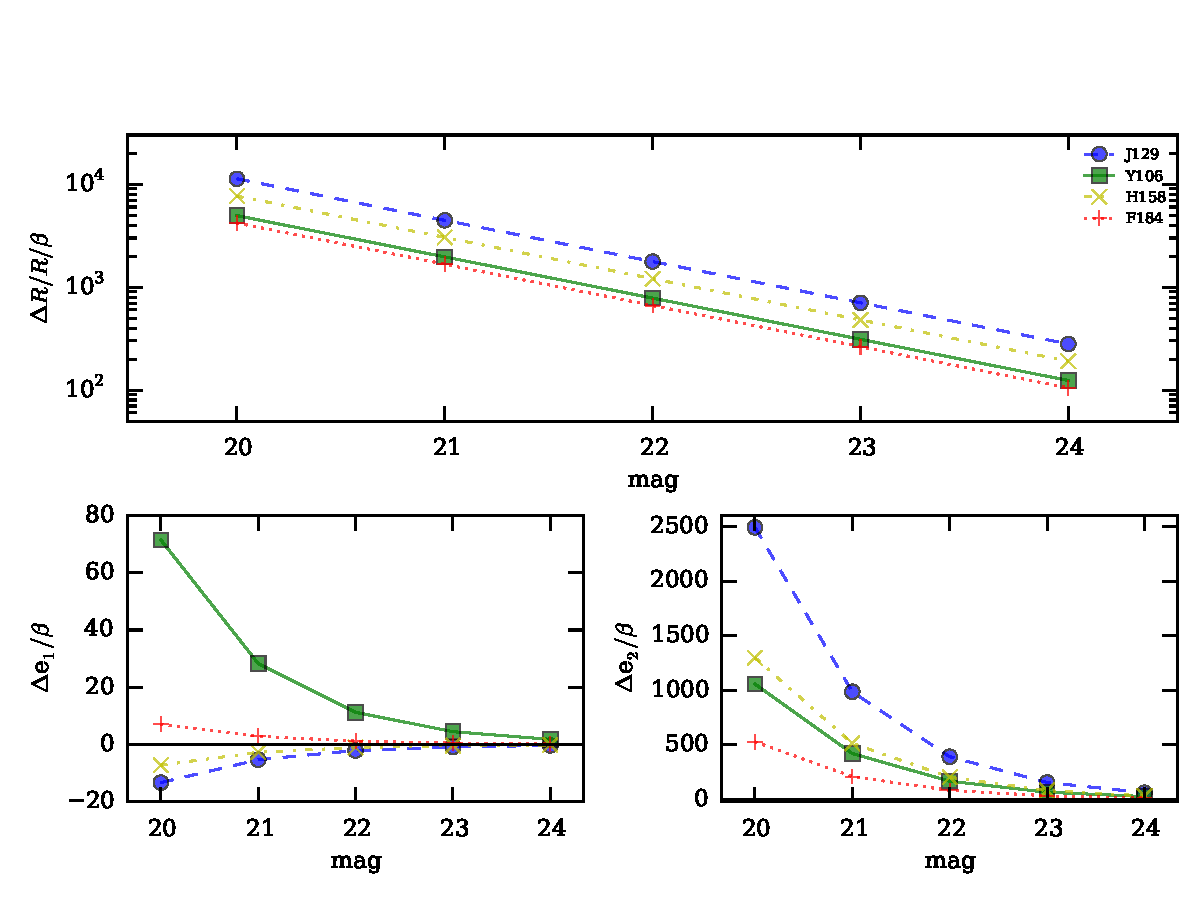
\includegraphics[page=1]{plots/delta_r_over_r_over_beta_delta_e_over_beta_vs_mag_wfirst_psf_10_realizations_12-19-2015.pdf}}
\caption{Fractional error in PSF size and absolute error in PSF ellipticity components normalized by the VNL parameter $\beta$, as a function of magnitude for the four HSL filters (J129, Y106, H158, and F184). The ordinate axis in each plot represents the slope of the linear relationships in Fig. \ref{beta}, derived by linear fitting of points around the vicinity of $\beta_0$ in each curve of that figure.}
\label{magnitude}
\end{figure}
\newpage
\section{Conclusion}
\label{Conclusion}
We have used the \wfa\ module in \gs\ to study the impact on PSF measurement for weak lensing science due to the non-linearity in the conversion of charge to voltage in near-infrared hybrid CMOS detectors (such as those that will be used in the Wide Field Imager of the \wfa\ mission). The PSF profiles created by {\tt{galsim.wfirst}} posses several of the design characteristics of the expected PSF of the mission, such as optical aberrations and pixel scale. We have also used the \wfa\ Exposure Time Calculator in Weak Lensing mode to assign the PSF profiles fluxes per pixel consistent with the expected brightness of the HSL. 

Voltage non-linearity--as studied in this work--encompasses the linearity due to the shrinking of the depletion region at the p-n junction as charge accumulates, and the deviation from linearity originating in the multiplexer gain. It depends on the total integrated signal (fluence), and it is more dominant at high signals than other types of non-linearity such as reciprocity failure, which dominate at lower signals. As such, VNL will tend to attenuate the bright stars that are usually used for PSF estimation, introducing errors when de-convolving the PSF at the interpolated galaxy positions.

To model VNL, we have used a single, one-parameter transfer function quadratic in the mean signal $\langle Q \rangle$ (Eq. \ref{vnl}). In principle, different pixels can have different underlying non-linearity coefficients which in practice can be difficult to measure with sufficient precision, so the mean response is usually measured. In our simulations, we have assumed that each individual pixel has a different non-linearity coefficient that follows a Normal distribution, and we have verified that the results obtained in this way do not differ from those obtained by using the mean VNL coefficient for all pixels. 

We have studied the impact of VNL in isolation by using the relationship in Eq.\ref{vnl},  not considering other sensor effects. We have used the metrics $\Delta R/R$ and $\Delta e$ to assess the impact of VNL on PSF size and ellipticity (which have to be controlled to $\sim O(10^{-3})$ or better), for different values of the parameter space at hand ($\beta$, PSF magnitude, and bandpass filter to be utilized in WL analyses). In particular, our simulations show that the effects of VNL are the largest in the J129 and linear with the nonlinearity parameter $\beta$. At the nominal value $\beta_0$, VNL induces errors in PSF size and shape comparable to what is required by accurate WL measurements. To limit these biases to the requirements, $\beta$ should be calibrated to about $3-5\%$. 


%Something to keep in mind is that different pixels could have different underlying linearity coefficients but in practice its very hard to measure this with sufficient precision so we find ourselves using the mean pixel behavior and accepting a degree of mismatch between a pixel and the mean.  Does this matter?   Maybe not, but I think this si a good example where simulation is better than measurement since you can test whether biases are introduced.   

%Nonlinear gain V(Q) depends on fluence (total charge/pixel), not flux (charge/pixel/second).  We can't use SPR to measure nonlinear gain because there's no independent measurement of Q.  We're not really measuring flux in the reciprocity failure case either, just a signal decay.

We thank \ldots
\section*{Appendix}
The parameters used in the weak lensing mode of the Exposure Time Calculator (ETC-WL) to obtain the flux (in electrons) at AB magnitude 20 for each of the four bands simulated (J129, W149, H158, and F184) are as follows: 
\begin{multicols}{2}
\begin{enumerate}
\item[-] telescope configuration: 0 (generic)
\item[-] aperture outer diameter: 2.4 m
\item[-] central obscuration: 0.3
\item[-] pixel scale: 0.11 arcsec/pix
\item[-] throughput: 0.8
\item[-] RMS wavefront error: 0.05 $\mu$m
\item[-] detector type: 2 (H4RG)
\item[-] pointing jitter: 0.00 arcsec per axis
\item[-] minimum wavelength: \emph{filter dependent} (see Table 1)
\item[-] maximum wavelength: \emph{filter dependent} (see Table 1)
\item[-] filter throughput: 0.99  
\item[-] single exposure time: 174 s
\item[-] readnoise floor: 0.0 e$^{-}$/pix/s
\item[-] dark current: 0.0 e$^{-}$/pix/s
\item[-] (heliocentric) ecliptic latitude: -30 deg
\item[-] galactic redenning E(B-V): 0.03 mag
\item[-] number of exposures: 36 ($N=6$) 
\item[-] minimum resolution factor R: 0.425
\item[-] maximum ellipticity error: 0.2
\end{enumerate}
\end{multicols}


%?Nonlinearity? includes nonlinear conversion gain (e-/ADU) and the ?brighter-fatter effect?. Postdoc Andres Plazas-Malagon is calculating the effects of these on shape measurement with WFIRST.
%Weak lensing scientists typically assume that nonlinear conversion gain (NL) will be sufficiently calibrated.  This was based on
%Experience with CCDs, not CMOS
%Previous, less stringent shape measurement requirements
%Top plot shows the change in PSF size DR/R vs. star magnitude for a single NL parameter b (quadratic term) in various filters.  For a nominal b=3.6E-7, NL biases the size of the brightest useable stars in the High Latitude Survey by a few \%.
%Bottom plot shows general relationship between size bias and b. To limit relative size bias of the brightest stars to ~10-4, b must be calibrated to better than 1\%.




\acknowledgments
%We thank...
\bibliographystyle{plainnat}
\bibliography{bias_from_NL}

\end{document}